
\section{Анализ и выделение основного направления производительности позиционного пневмопривода}\label{sec:ch1/sec2}

Классификация пневмоприводов может осуществляться по нескольким ключевым критериям,
таким как тип движения объекта регулирования и способ управления.
На основе этих критериев ПП подразделяются на два основных типа:
цикловые и следящие. Особый интерес представляет подкатегория следящих
ПП --- позиционные приводы.
Рисунок  \ref*{fig:actuators_scheme} иллюстрирует схему классификации
ПП согласно указанным критериям.


\begin{figure}[ht]
    \centerfloat{
        \begin{tikzpicture}
            \usetikzlibrary {positioning,shapes.misc,arrows}
            \tikzstyle{block} = [rectangle, draw, text centered, minimum height=4em, line width=1pt]
            \tikzstyle{arr} = [-triangle 45, line width=1pt]
            \node [block] (pneumatic) {Пневмопривод};
            \node [block, below=1.5cm of pneumatic, xshift=-2cm] (cycle) {Цикловой};
            \node [block, below=1.5cm of pneumatic, xshift=2cm] (tracking) {Следящий};
            \node [block, below=1.5cm of tracking] (positioning) {Позиционный};

            \draw[arr] (pneumatic.south) -- ++(0,-1) -| (cycle);
            \draw[arr] (pneumatic.south) -- ++(0,-1) -| (tracking);
            \draw[arr] (tracking.south) -- ++(0,-1) -| (positioning);
        \end{tikzpicture}
    }
    \caption{Классификация пневмопривода}\label{fig:actuators_scheme}
\end{figure}

Одним из первых исследователей поизиционных ПП является Филлипов И. Б.
В своей работе \cite*{филиппов:позиц_след_пневмопривод}
автор рассматривает вопрос расширения функциональных возможностей промышленных роботов,
оснащенных ПП, за счет внедрения в их конструкцию принципиально
новой схемы ПП с переменной структурой. Предлагаемая автором система привода способна
работать в двух различных режимах - релейном и следящем. Предлагаемая структура представлена на рисунке \ref*{fig:phillipov_positioning}

\begin{figure}[h]
    \centerfloat
    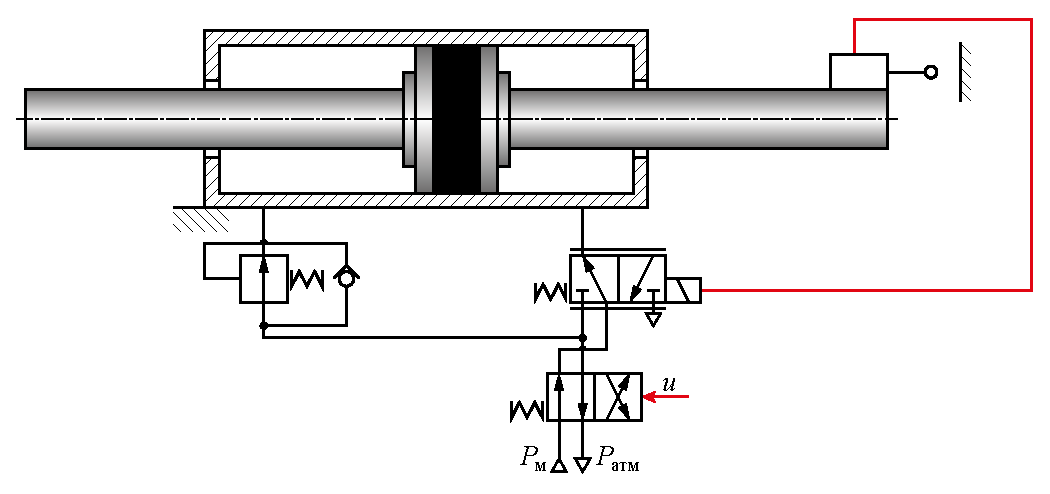
\includegraphics{phillipov_pp.eps}
    \caption{Типовая схема следящего пневмопривода}\label{fig:phillipov_positioning}
\end{figure}

На участках разгона и установившегося движения рабочего органа промышленного робота
ПП функционирует в релейном режиме, аналогично традиционным решениям.
Однако при осуществлении торможения и точного позиционирования привод переключается в
следящий режим работы. Это достигается путем введения в схему дополнительных элементов,
таких как пропорциональный распределитель и датчик обратной связи, установленный непосредственно
на РО.

Ключевой особенностью предлагаемой автором конструкции пневмопривода является возможность
позиционирования рабочего органа в любой точке по ходу поршня пневмоцилиндра. В отличие от
традиционных приводов, имеющих ограниченное число точек позиционирования, в данной схеме параметры
привода, такие как давления, расходы и объемы полостей, могут изменяться в зависимости от текущей
координаты поршня в точке позиционирования.

Автором упоминается, что к позиционным приводам, в том числе пневматическим с
позиционированием в следящем режиме, предъявляются ключевые требования, связанные с
обеспечением высокой точности остановки рабочего органа в заданной точке, устойчивости
состояния равновесия и минимального перерегулирования при торможении \cite*{shortnikov:a}.
Данные требования
к качеству переходного процесса были учтены автором при исследовании динамики предлагаемого
пневмопривода с переменной структурой.

Таким образом можно утверждать, что точки зрения схемотехники, позиционные ПП идентичны следящим
и также способны отслеживать непрерывный входной сигнал.
И в современных реалиях для этой цели используются специальные пропорциональные распределители, золотник которых
может занимать промежуточные положения. Подобные системы отличаются большей сложностью и,
соответственно, более высокой стоимостью. Они обеспечивают точное воспроизведение движения
объекта регулирования в соответствии с заданным алгоритмом. Вероятность ошибки при отработке
заданной траектории ограничивается точностью и быстродействием измерительных и управляющих
устройств, а также алгоритмом управления. Основными элементами системы являются:

\begin{enumerate}
    \item Датчики снимающие те или иные физические параметры пневмопривода
          (положение объекта регулирования, давления в полостях пневмодвигателя и т. д.) в процессе работы;
    \item Системы сбора информации и электронно-вычислительные устройства задающие управляющий сигнал для
          регулирующего оборудования;
    \item Исполнительное оборудование выполняющее перемещение объекта регулирования (пневмомоторы, пневмоцилиндры);
    \item Направляющее и регулирующее оборудование (распределители, клапана и т. д.);
    \item Энергообеспечивающие устройства (компрессорные станции, устройства подготовки воздуха).
\end{enumerate}

На рисунке \ref*{fig:template_pneumatic_actuator} представлена типовая схема следящего пневмопривода.

\begin{figure}[h]
    \centerfloat
    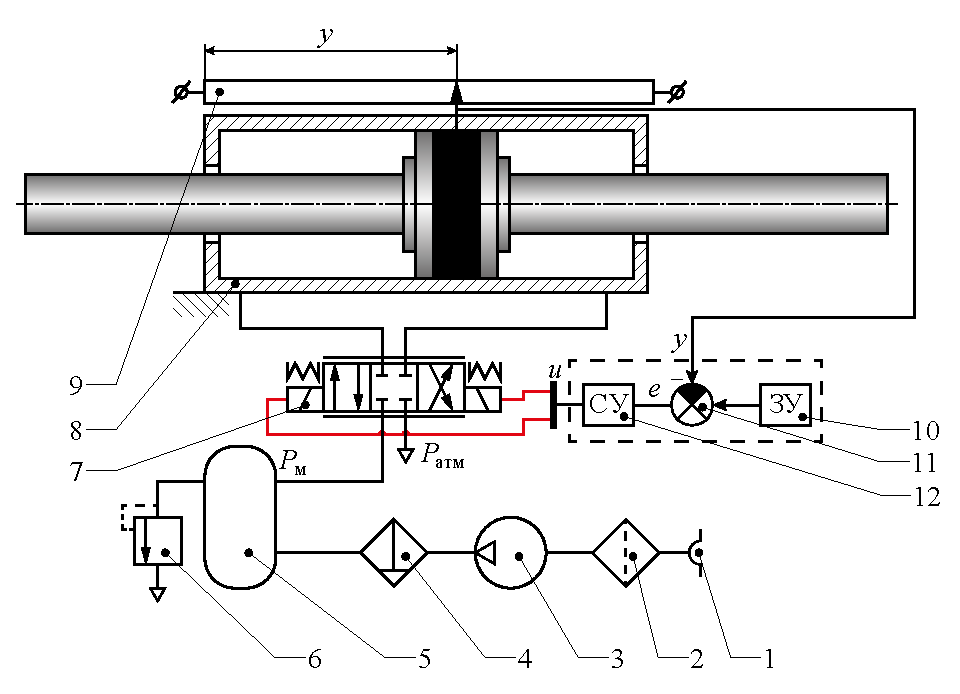
\includegraphics{follow_actuator.eps}
    \caption{Типовая схема следящего пневмопривода}\label{fig:template_pneumatic_actuator}
\end{figure}
На представленом выше рисунке \ref*{fig:actuators_scheme}: 1 --- воздухозабор; 2 --- воздушный фильтр; 3 --- компрессор;
4 --- влаго- маслоотделитель; 5 --- ресивер; 6 --- предохранительный клапан; 7 --- пропорциональный
распределитель 4/3; 8 --- пневмоцилиндр; 9 --- потенциометрический датчик положения;
10 --- задающее устройство; 11 --- сравнивающее устройство; 12 --- система управления.

Однако для позиционных пневмоприводов, задача которых заключается в
позиционировании в заданной координате без отработки определенной траектории,
использование такой структуры является избыточным. В этом случае целесообразно
упрощение схемы за счет применения дискретных распределителей. Один из возможных вариантов исполнения пневмопривода
с дискретным управлением показан на рисунке
\ref*{fig:template_discrete_pneumatic_actuator}.

\begin{figure}[h]
    \centerfloat
    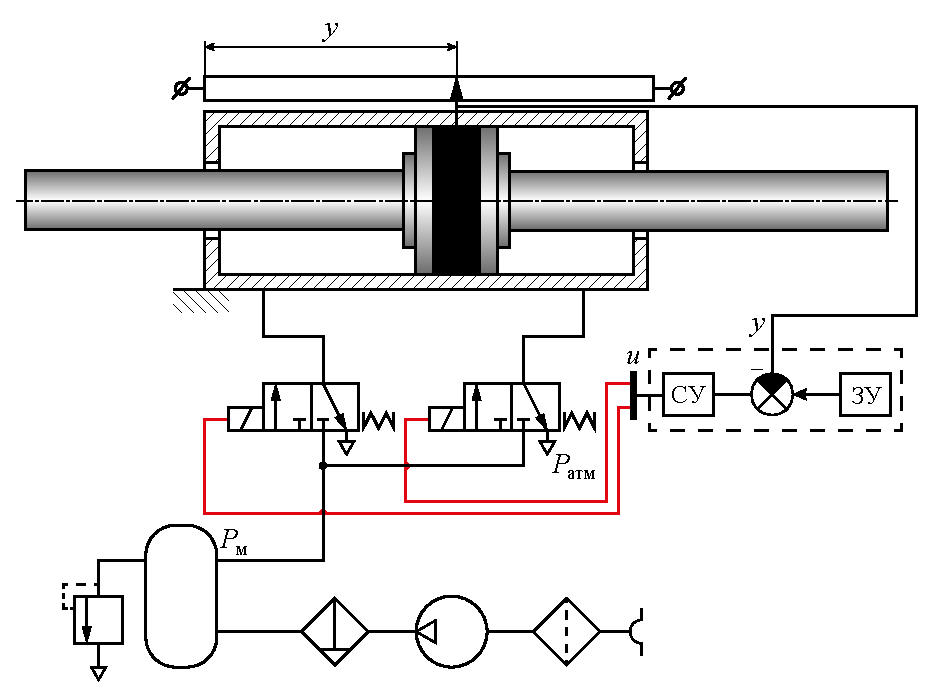
\includegraphics{positioning_actuator.eps}
    \caption{Типовая схема позиционного пневмопривода с дискретным управлением}\label{fig:template_discrete_pneumatic_actuator}
\end{figure}

Поскольку, как было упомянуто ранее, нет необходимости отрабатывать конкретную траекторию движения,
то на рисунке \ref*{fig:ideal_vel_process} можно представить идеализированный процесс позиционирования ОР [].

\begin{figure}[h]
    \centerfloat
    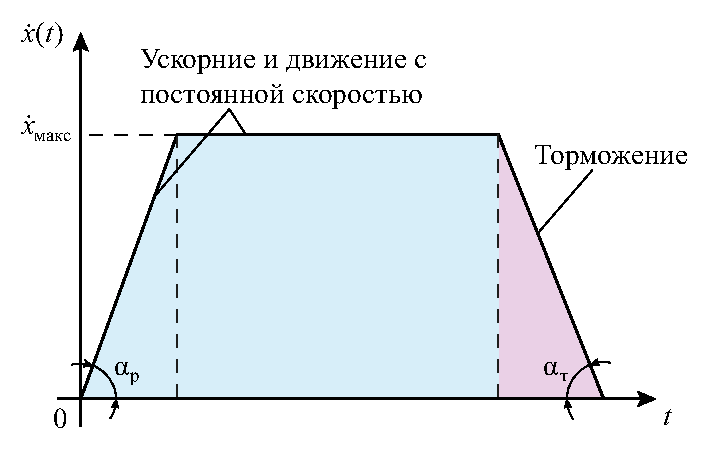
\includegraphics{ideal_vel_process.eps}
    \caption{Идеализированный закон движения РО}\label{fig:ideal_vel_process}
\end{figure}


Согласно представленному рисунку видно, что идеализированный процесс позиционирования состоит из трех этапов:

\begin{enumerate}
    \item разгон с постоянным ускорением;
    \item движение с постоянной скоростью;
    \item торможение с постоянным ускорением.
\end{enumerate}

Основополагающими этапами, которые определяют быстродействие системы, являются --- этап разгона
до максимальной скорости и этап торможения до точки позиционирования.

Чтобы оптимизировать работу позиционного ПП и повысить его эффективность,
необходимо детально рассмотреть каждый из этих ключевых этапов.
Анализ особенностей разгона до максимальной скорости и торможения
до точки позиционирования позволит выявить потенциальные области для
улучшения и определить наиболее подходящие методы и подходы для достижения
оптимальной производительности системы.

Разберём подробно данные основополагающие этапы,
уделяя особое внимание факторам, влияющим на быстродействие системы,
а также рассмотрим возможные пути повышения эффективности каждого этапа.
Это позволит сформировать целостное представление о функционировании позиционного ПП и
определить наиболее перспективные направления совершенствования.
